\chapter{Modellering}
I projektet er der opgivet data for en "typisk" dag i form af et skema over hyppigheden af ankomsttider mellem fly og hyppigheden af landingsvarigheden for fly. For at kunne lave en simulering af flyankomster i en dag i lufthavnen, er det nødvendigt at analysere denne data, og eventuelt finde en model til at generere tiderne, som stemmer overens med den "typiske" dag.
\section{Ankomsttider}
Givet er data for hvor mange fly der ankommer inden for et specifikt interval efter det forrige fly. På baggrund af dette kan der genereres ankomsttider for en specifik dag det første år, og tiden det tager for alle fly at ankomme kan da beregnes.

En måde at gøre det på er, at generere først $44$ tilfældige tal mellem $0 - 59$, så $34$ tilfældige tal mellem $60 - 119$, osv. Alle disse ankomstider mellem flyene kan da lægges sammen, og denne sum må da være den tid det tager for alle 200 fly at ankomme.
I filen \code{arrival\_times.py} kan man se et \textsc{Python}-program der gør netop dette, og som printer antallet af fly og tiden i alt i timer.
Køres dette et par gange vil resultatet være, at der alle gange er 200 fly, men at tiden i alt vil varriere mellem $12 - 13.5$ timer.

Da tiden i alt varrierer, vælges det at køre programmet mange gange for da at tage gennemsnittet af alle kørsler.
I filen \code{arrival\_times\_mean.py} findes et \textsc{Python}-program der udfører netop dette, og som printer gennemsnittet. Køres dette program $100,000$ gange (ved at sætte variablen \code{repetitions = 100000}) fås et gennemsnit på $12.9$ timer.

\subsection{Model for ankomsttider} \label{chap:model_arrival_times}
Det kunne forestilles, at fly i en lufthavn ankommer uafhængigt af hinanden i løbet af den tid lufthavnen tager imod ankomster.
Derfor kunne en passende model måske være at ankomsttiderne er tilfældigt spredt på en tidslinje på $13$ timer.
Denne hypotese kan undersøges.
I programmet \code{plot\_inter\_arrival\_time\_model.py} gerereres der $200$ tilfældige sekunder i tidsintervallet fra $0 - 13$ timer, der så sorteres. Dette må være en liste over ankomstiderne med denne model.
Da udregnes ankomsttiderne mellem flyene, og der tælles op, hvor mange ankomsttider mellem flyene der er i de givne intervaller.
Dette gentages mange gange, og der bliver taget en gennemsnit af alle antallene hvilket til sidst plottes.

I Figur \ref{fig:given_arrival_time_plot} ses de givne data for ankomsttider på en typisk dag plottet i et histogram, mens der i Figur \ref{fig:model_arrival_time_plot} ses gennemsnittet for de genererede ankomsttider med modellen plottet i et histogram.

\begin{figure}[h!]
	\centering
	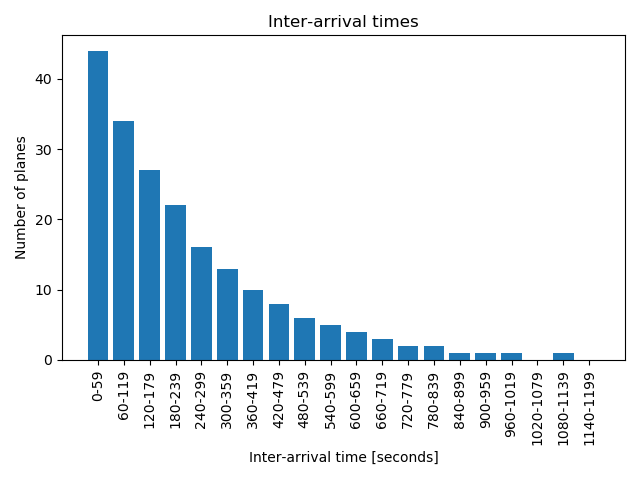
\includegraphics[scale=0.7]{fig/img/given_arrival_time_plot.png}
	\caption{Plot over det givne datasæt for ankomsttimer} \label{fig:given_arrival_time_plot}
\end{figure}

\begin{figure}[h!]
	\centering
	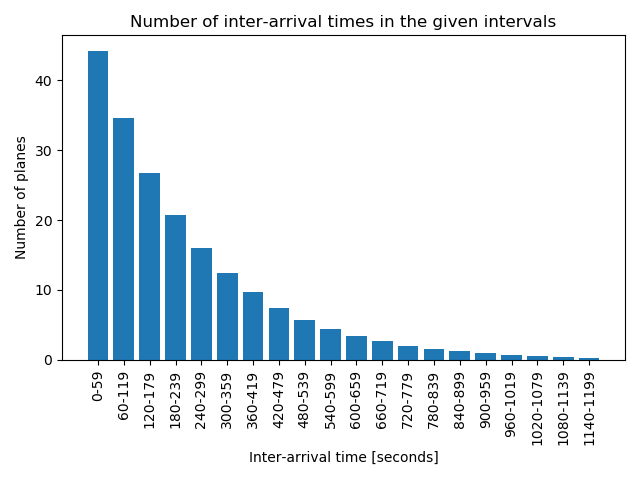
\includegraphics[scale=0.7]{fig/img/model_arrival_time_plot.png}
	\caption{Plot over gennemsnittet af antal for de generede ankomsttimer med modellen} \label{fig:model_arrival_time_plot}
\end{figure}

Det er tydeligt at modellen er god for ankomsttiderne. Da må ankomsttiderne for flyvemaskinerne i lufthavnen kunne simuleres, ved tilfældigt at plotte dem på en tidslinje fra $0 - 13$ timer.

\section{Landingsvarigheder}
Landingsvarighed er den tid (i sekunder) et fly bruger på at lande.
Altså er landingsbanen fri når landingsvarighed for et fly er gået.
Igen er det givne data for en "typisk" dag en tabel over tidsintervaller, og det antal fly hvis landingsvarighed ligger inden for det. Igen summerer antallet af fly til 200. I Figur \ref{fig:given_landing_durations_plot} ses et histogram over antallet af fly og landingsvarighederne.

\begin{figure}[h!]
	\centering
	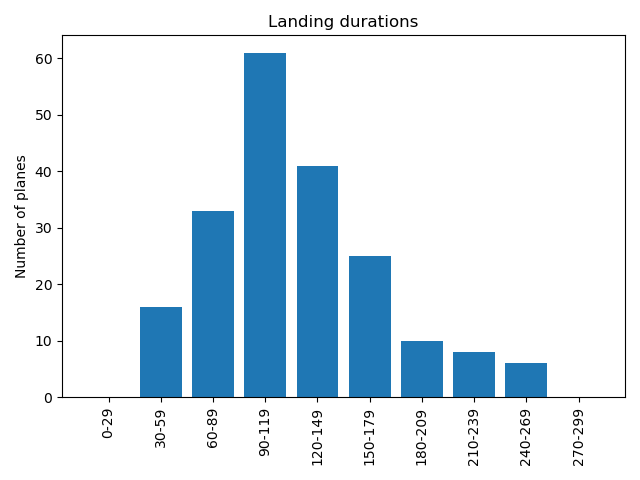
\includegraphics[scale=0.6]{fig/img/given_landing_durations_plot.png}
	\caption{Plot over det give data for landingsvarighederne.} \label{fig:given_landing_durations_plot}
\end{figure}

Det ses i Figur \ref{fig:given_landing_durations_plot} at fordelingen er forskellig fra ankomsttiderne.
Fordelingen ligner til dels en normalfordeling, da der på samme måde som i en normalfordeling er en "pukkel".
Dog er fordeligen for landingsvarighederne ikke symmetrisk omkring det højeste punkt, som en normalfordeling er, og ligner derfor mere en "skæv" normalfordeling.

Det har i projektet ikke været muligt at finde en model der passer på det givne data.
Desuden afviger landingsvarighederne sig fra ankomsttiderne, da landingsvarigheden direkte kan blive påvirket af udefrakommende paramentre.
Landingsvarigheden for et fly vil ikke bare være et tilfældigt tal inden for et tidsinterval, men vil kunne blive påvirket af eksempelvis den hastighed eller acceleration flyet lander med. 

Da der ikke er blevet fundet en model der passer til det givne data, må det blive nødvendigt at bruge netop de givne tidsintervaller til at generere tilfældige landingsvarigheder for en specifik dag. Den specifikke metode brugt i dette projekt beskrives i afsnit \ref{chap:landing_durations} i kapitel \ref{chap:program}.
